%% bare_conf.tex
%% V1.4b
%% 2015/08/26
%% by Michael Shell
%% See:
%% http://www.michaelshell.org/
%% for current contact information.
%%
%% This is a skeleton file demonstrating the use of IEEEtran.cls
%% (requires IEEEtran.cls version 1.8b or later) with an IEEE
%% conference paper.
%%
%% Support sites:
%% http://www.michaelshell.org/tex/ieeetran/
%% http://www.ctan.org/pkg/ieeetran
%% and
%% http://www.ieee.org/

%%*************************************************************************
%% Legal Notice:
%% This code is offered as-is without any warranty either expressed or
%% implied; without even the implied warranty of MERCHANTABILITY or
%% FITNESS FOR A PARTICULAR PURPOSE!
%% User assumes all risk.
%% In no event shall the IEEE or any contributor to this code be liable for
%% any damages or losses, including, but not limited to, incidental,
%% consequential, or any other damages, resulting from the use or misuse
%% of any information contained here.
%%
%% All comments are the opinions of their respective authors and are not
%% necessarily endorsed by the IEEE.
%%
%% This work is distributed under the LaTeX Project Public License (LPPL)
%% ( http://www.latex-project.org/ ) version 1.3, and may be freely used,
%% distributed and modified. A copy of the LPPL, version 1.3, is included
%% in the base LaTeX documentation of all distributions of LaTeX released
%% 2003/12/01 or later.
%% Retain all contribution notices and credits.
%% ** Modified files should be clearly indicated as such, including  **
%% ** renaming them and changing author support contact information. **
%%*************************************************************************


% *** Authors should verify (and, if needed, correct) their LaTeX system  ***
% *** with the testflow diagnostic prior to trusting their LaTeX platform ***
% *** with production work. The IEEE's font choices and paper sizes can   ***
% *** trigger bugs that do not appear when using other class files.       ***                          ***
% The testflow support page is at:
% http://www.michaelshell.org/tex/testflow/



\documentclass[conference]{IEEEtran}
% Some Computer Society conferences also require the compsoc mode option,
% but others use the standard conference format.
%
% If IEEEtran.cls has not been installed into the LaTeX system files,
% manually specify the path to it like:
% \documentclass[conference]{../sty/IEEEtran}





% Some very useful LaTeX packages include:
% (uncomment the ones you want to load)


% *** MISC UTILITY PACKAGES ***
%
%\usepackage{ifpdf}
% Heiko Oberdiek's ifpdf.sty is very useful if you need conditional
% compilation based on whether the output is pdf or dvi.
% usage:
% \ifpdf
%   % pdf code
% \else
%   % dvi code
% \fi
% The latest version of ifpdf.sty can be obtained from:
% http://www.ctan.org/pkg/ifpdf
% Also, note that IEEEtran.cls V1.7 and later provides a builtin
% \ifCLASSINFOpdf conditional that works the same way.
% When switching from latex to pdflatex and vice-versa, the compiler may
% have to be run twice to clear warning/error messages.






% *** CITATION PACKAGES ***
%
%\usepackage{cite}
% cite.sty was written by Donald Arseneau
% V1.6 and later of IEEEtran pre-defines the format of the cite.sty package
% \cite{} output to follow that of the IEEE. Loading the cite package will
% result in citation numbers being automatically sorted and properly
% "compressed/ranged". e.g., [1], [9], [2], [7], [5], [6] without using
% cite.sty will become [1], [2], [5]--[7], [9] using cite.sty. cite.sty's
% \cite will automatically add leading space, if needed. Use cite.sty's
% noadjust option (cite.sty V3.8 and later) if you want to turn this off
% such as if a citation ever needs to be enclosed in parenthesis.
% cite.sty is already installed on most LaTeX systems. Be sure and use
% version 5.0 (2009-03-20) and later if using hyperref.sty.
% The latest version can be obtained at:
% http://www.ctan.org/pkg/cite
% The documentation is contained in the cite.sty file itself.






% *** GRAPHICS RELATED PACKAGES ***
%
\ifCLASSINFOpdf
  % \usepackage[pdftex]{graphicx}
  % declare the path(s) where your graphic files are
  % \graphicspath{{../pdf/}{../jpeg/}}
  % and their extensions so you won't have to specify these with
  % every instance of \includegraphics
  % \DeclareGraphicsExtensions{.pdf,.jpeg,.png}
\else
  % or other class option (dvipsone, dvipdf, if not using dvips). graphicx
  % will default to the driver specified in the system graphics.cfg if no
  % driver is specified.
  % \usepackage[dvips]{graphicx}
  % declare the path(s) where your graphic files are
  % \graphicspath{{../eps/}}
  % and their extensions so you won't have to specify these with
  % every instance of \includegraphics
  % \DeclareGraphicsExtensions{.eps}
\fi
% graphicx was written by David Carlisle and Sebastian Rahtz. It is
% required if you want graphics, photos, etc. graphicx.sty is already
% installed on most LaTeX systems. The latest version and documentation
% can be obtained at:
% http://www.ctan.org/pkg/graphicx
% Another good source of documentation is "Using Imported Graphics in
% LaTeX2e" by Keith Reckdahl which can be found at:
% http://www.ctan.org/pkg/epslatex
%
% latex, and pdflatex in dvi mode, support graphics in encapsulated
% postscript (.eps) format. pdflatex in pdf mode supports graphics
% in .pdf, .jpeg, .png and .mps (metapost) formats. Users should ensure
% that all non-photo figures use a vector format (.eps, .pdf, .mps) and
% not a bitmapped formats (.jpeg, .png). The IEEE frowns on bitmapped formats
% which can result in "jaggedy"/blurry rendering of lines and letters as
% well as large increases in file sizes.
%
% You can find documentation about the pdfTeX application at:
% http://www.tug.org/applications/pdftex





% *** MATH PACKAGES ***
%
%\usepackage{amsmath}
% A popular package from the American Mathematical Society that provides
% many useful and powerful commands for dealing with mathematics.
%
% Note that the amsmath package sets \interdisplaylinepenalty to 10000
% thus preventing page breaks from occurring within multiline equations. Use:
%\interdisplaylinepenalty=2500
% after loading amsmath to restore such page breaks as IEEEtran.cls normally
% does. amsmath.sty is already installed on most LaTeX systems. The latest
% version and documentation can be obtained at:
% http://www.ctan.org/pkg/amsmath





% *** SPECIALIZED LIST PACKAGES ***
%
%\usepackage{algorithmic}
% algorithmic.sty was written by Peter Williams and Rogerio Brito.
% This package provides an algorithmic environment fo describing algorithms.
% You can use the algorithmic environment in-text or within a figure
% environment to provide for a floating algorithm. Do NOT use the algorithm
% floating environment provided by algorithm.sty (by the same authors) or
% algorithm2e.sty (by Christophe Fiorio) as the IEEE does not use dedicated
% algorithm float types and packages that provide these will not provide
% correct IEEE style captions. The latest version and documentation of
% algorithmic.sty can be obtained at:
% http://www.ctan.org/pkg/algorithms
% Also of interest may be the (relatively newer and more customizable)
% algorithmicx.sty package by Szasz Janos:
% http://www.ctan.org/pkg/algorithmicx




% *** ALIGNMENT PACKAGES ***
%
%\usepackage{array}
% Frank Mittelbach's and David Carlisle's array.sty patches and improves
% the standard LaTeX2e array and tabular environments to provide better
% appearance and additional user controls. As the default LaTeX2e table
% generation code is lacking to the point of almost being broken with
% respect to the quality of the end results, all users are strongly
% advised to use an enhanced (at the very least that provided by array.sty)
% set of table tools. array.sty is already installed on most systems. The
% latest version and documentation can be obtained at:
% http://www.ctan.org/pkg/array


% IEEEtran contains the IEEEeqnarray family of commands that can be used to
% generate multiline equations as well as matrices, tables, etc., of high
% quality.




% *** SUBFIGURE PACKAGES ***
%\ifCLASSOPTIONcompsoc
%  \usepackage[caption=false,font=normalsize,labelfont=sf,textfont=sf]{subfig}
%\else
%  \usepackage[caption=false,font=footnotesize]{subfig}
%\fi
% subfig.sty, written by Steven Douglas Cochran, is the modern replacement
% for subfigure.sty, the latter of which is no longer maintained and is
% incompatible with some LaTeX packages including fixltx2e. However,
% subfig.sty requires and automatically loads Axel Sommerfeldt's caption.sty
% which will override IEEEtran.cls' handling of captions and this will result
% in non-IEEE style figure/table captions. To prevent this problem, be sure
% and invoke subfig.sty's "caption=false" package option (available since
% subfig.sty version 1.3, 2005/06/28) as this is will preserve IEEEtran.cls
% handling of captions.
% Note that the Computer Society format requires a larger sans serif font
% than the serif footnote size font used in traditional IEEE formatting
% and thus the need to invoke different subfig.sty package options depending
% on whether compsoc mode has been enabled.
%
% The latest version and documentation of subfig.sty can be obtained at:
% http://www.ctan.org/pkg/subfig




% *** FLOAT PACKAGES ***
%
%\usepackage{fixltx2e}
% fixltx2e, the successor to the earlier fix2col.sty, was written by
% Frank Mittelbach and David Carlisle. This package corrects a few problems
% in the LaTeX2e kernel, the most notable of which is that in current
% LaTeX2e releases, the ordering of single and double column floats is not
% guaranteed to be preserved. Thus, an unpatched LaTeX2e can allow a
% single column figure to be placed prior to an earlier double column
% figure.
% Be aware that LaTeX2e kernels dated 2015 and later have fixltx2e.sty's
% corrections already built into the system in which case a warning will
% be issued if an attempt is made to load fixltx2e.sty as it is no longer
% needed.
% The latest version and documentation can be found at:
% http://www.ctan.org/pkg/fixltx2e


%\usepackage{stfloats}
% stfloats.sty was written by Sigitas Tolusis. This package gives LaTeX2e
% the ability to do double column floats at the bottom of the page as well
% as the top. (e.g., "\begin{figure*}[!b]" is not normally possible in
% LaTeX2e). It also provides a command:
%\fnbelowfloat
% to enable the placement of footnotes below bottom floats (the standard
% LaTeX2e kernel puts them above bottom floats). This is an invasive package
% which rewrites many portions of the LaTeX2e float routines. It may not work
% with other packages that modify the LaTeX2e float routines. The latest
% version and documentation can be obtained at:
% http://www.ctan.org/pkg/stfloats
% Do not use the stfloats baselinefloat ability as the IEEE does not allow
% \baselineskip to stretch. Authors submitting work to the IEEE should note
% that the IEEE rarely uses double column equations and that authors should try
% to avoid such use. Do not be tempted to use the cuted.sty or midfloat.sty
% packages (also by Sigitas Tolusis) as the IEEE does not format its papers in
% such ways.
% Do not attempt to use stfloats with fixltx2e as they are incompatible.
% Instead, use Morten Hogholm'a dblfloatfix which combines the features
% of both fixltx2e and stfloats:
%
% \usepackage{dblfloatfix}
% The latest version can be found at:
% http://www.ctan.org/pkg/dblfloatfix




% *** PDF, URL AND HYPERLINK PACKAGES ***
%
%\usepackage{url}
% url.sty was written by Donald Arseneau. It provides better support for
% handling and breaking URLs. url.sty is already installed on most LaTeX
% systems. The latest version and documentation can be obtained at:
% http://www.ctan.org/pkg/url
% Basically, \url{my_url_here}.




% *** Do not adjust lengths that control margins, column widths, etc. ***
% *** Do not use packages that alter fonts (such as pslatex).         ***
% There should be no need to do such things with IEEEtran.cls V1.6 and later.
% (Unless specifically asked to do so by the journal or conference you plan
% to submit to, of course. )


% correct bad hyphenation here
\hyphenation{op-tical net-works semi-conduc-tor}
\usepackage{graphicx}
\usepackage{amssymb}
%\usepackage{subfigure}
\usepackage{xspace}
\usepackage[british,UKenglish,USenglish,english,american]{babel}
\usepackage{color}
\usepackage{tikz}
\usepackage{listings}
\usepackage{etoolbox}
\usepackage{subfig}
\usepackage{url}
%\usepackage[caption=false,font=footnotesize]{subfig}


\newcommand{\circled}[2][]{\tikz[baseline=(char.base)]
    {\node[shape = circle, draw, inner sep = 1pt]
    (char) {\phantom{\ifblank{#1}{#2}{#1}}};%
    \node at (char.center) {\makebox[0pt][c]{#2}};}}
\robustify{\circled}


\newcommand{\tabincell}[2]{\begin{tabular}{@{}#1@{}}#2\end{tabular}}
\newcommand{\DSVMP}{\textsc{Dsvmp}\xspace}

\IEEEoverridecommandlockouts

\renewcommand{\thefootnote}{\fnsymbol{footnote}}

\newcommand\FIXME[1]{\textcolor{red}{FIX:}\textcolor{red}{#1}}

\lstdefinelanguage
   [x64]{Assembler}     % add a "x64" dialect of Assembler
   [x86masm]{Assembler} % based on the "x86masm" dialect
   % with these extra keywords:
   {morekeywords={CDQE,CQO,CMPSQ,CMPXCHG16B,JRCXZ,LODSQ,MOVSXD, %
                  POPFQ,PUSHFQ,SCASQ,STOSQ,IRETQ,RDTSCP,SWAPGS, %
                  rax,rdx,rcx,rbx,rsi,rdi,rsp,rbp, %
                  r8,r8d,r8w,r8b,r9,r9d,r9w,r9b}} % etc
\lstset{language=[x64]Assembler}


\definecolor{codegreen}{rgb}{0,0.6,0}
\definecolor{codegray}{rgb}{0.5,0.5,0.5}
\definecolor{codepurple}{rgb}{0.58,0,0.82}
\definecolor{backcolour}{rgb}{0.95,0.95,0.92}

\lstdefinestyle{mystyle}{
    backgroundcolor=\color{backcolour},
    commentstyle=\color{codegreen},
    keywordstyle=\color{magenta},
    numberstyle=\tiny\color{codegray},
    stringstyle=\color{codepurple},
    basicstyle=\footnotesize,
    breakatwhitespace=false,
    breaklines=true,
    captionpos=b,
    keepspaces=true,
    numbers=left,
    numbersep=5pt,
    showspaces=false,
    showstringspaces=false,
    showtabs=false,
    tabsize=2
}

\lstset{style=mystyle}

%\def\@IEEEsectpunct{.\ \,}
%\def\paragraph{\@startsection{paragraph}{4}{\z@}{1.5ex plus 1.5ex minus 0.5ex}%
%{0ex}{\normalfont\normalsize\sffamily\bfseries}}
\makeatother

\begin{document}

%
\title{Exploiting Dynamic Scheduling for VM-Based Code Obfuscation}


\author{\IEEEauthorblockN{Kaiyuan Kuang\IEEEauthorrefmark{2}, Zhanyong Tang\IEEEauthorrefmark{2}\IEEEauthorrefmark{1}\thanks{*Corresponding author. Email address: zytang@nwu.edu.cn}, Xiaoqing Gong\IEEEauthorrefmark{2}, Dingyi Fang\IEEEauthorrefmark{2}, Xiaojiang Chen\IEEEauthorrefmark{2},\\
Tianzhang Xing\IEEEauthorrefmark{2}, Guixin Ye\IEEEauthorrefmark{2}, Jie Zhang\IEEEauthorrefmark{2}, Zheng Wang\IEEEauthorrefmark{3}}
\IEEEauthorblockA{\IEEEauthorrefmark{2}School of Information Science and Technology, Northwest University, Xi'an, 710127, P.R. China.\\
\IEEEauthorrefmark{3}School of Computing and Communications, Lancaster University, UK\\
%\IEEEauthorrefmark{2}\{xx, zytang, xiaoqinggong, dyf, ...\}@nwu.edu.cn, \IEEEauthorrefmark{3}z.wang@lancaster.ac.uk
}
%NWU-Irdeto IoT-Information Security Joint Laboratory\\
%$^*$Correspondence should be addressed to Zhanyong Tang, Email: zytang@nwu.edu.cn}
}
%\and
%\IEEEauthorblockN{Homer Simpson}
%\IEEEauthorblockA{Twentieth Century Fox\\
%Springfield, USA\\
%Email: homer@thesimpsons.com}
%\and
%\IEEEauthorblockN{James Kirk\\ and Montgomery Scott}
%\IEEEauthorblockA{Starfleet Academy\\
%San Francisco, California 96678--2391\\
%Telephone: (800) 555--1212\\
%Fax: (888) 555--1212}

% conference papers do not typically use \thanks and this command
% is locked out in conference mode. If really needed, such as for
% the acknowledgment of grants, issue a \IEEEoverridecommandlockouts
% after \documentclass

% for over three affiliations, or if they all won't fit within the width
% of the page, use this alternative format:
%
%\author{\IEEEauthorblockN{Michael Shell\IEEEauthorrefmark{1},
%Homer Simpson\IEEEauthorrefmark{2},
%James Kirk\IEEEauthorrefmark{3},
%Montgomery Scott\IEEEauthorrefmark{3} and
%Eldon Tyrell\IEEEauthorrefmark{4}}
%\IEEEauthorblockA{\IEEEauthorrefmark{1}School of Electrical and Computer Engineering\\
%Georgia Institute of Technology,
%Atlanta, Georgia 30332--0250\\ Email: see http://www.michaelshell.org/contact.html}
%\IEEEauthorblockA{\IEEEauthorrefmark{2}Twentieth Century Fox, Springfield, USA\\
%Email: homer@thesimpsons.com}
%\IEEEauthorblockA{\IEEEauthorrefmark{3}Starfleet Academy, San Francisco, California 96678-2391\\
%Telephone: (800) 555--1212, Fax: (888) 555--1212}
%\IEEEauthorblockA{\IEEEauthorrefmark{4}Tyrell Inc., 123 Replicant Street, Los Angeles, California 90210--4321}}




% use for special paper notices
%\IEEEspecialpapernotice{(Invited Paper)}




% make the title area
\maketitle

% As a general rule, do not put math, special symbols or citations
% in the abstract
\begin{abstract}
\par Code virtualization building upon virtual machine (VM) technologies is
emerging as a viable method for implementing code obfuscation to protect
programs against unauthorized analysis. State-of-the-art VM-based
protection approaches use a fixed scheduling structure where the
program follows a single, static execution path for the same input. Such
approaches, however, are vulnerable to certain scenarios where the
attacker can reuse knowledge extracted from previously seen software
to crack applications using similar protection schemes. This paper
presents \DSVMP, a novel VM-based code obfuscation approach for software protection.
\DSVMP brings together two techniques to provide stronger
code protection than prior VM-based schemes.
Firstly, it uses a dynamic instruction
scheduler to randomly direct the program to execute different paths without
violating the correctness across different runs. By randomly choosing
the program execution paths, the application exposes diverse behavior, making
it much more difficult for an attacker to reuse the knowledge collected from
previous runs or similar applications to perform attacks. Secondly, it employs
multiple VMs to further obfuscate the relationship between VM bytecode and
their interpreters, making code analysis even harder. We have implemented
\DSVMP  in a prototype system and evaluated it using a set of widely used applications.
Experimental results show that \DSVMP provides stronger protection with comparable runtime overhead
and code size when compared to two commercial VM-based code obfuscation tools.
\end{abstract}

\begin{IEEEkeywords}
Code virtualization; Code Obfuscation; Dynamic cumulative attack
\end{IEEEkeywords}
% no keywords




% For peer review papers, you can put extra information on the cover
% page as needed:
% \ifCLASSOPTIONpeerreview
% \begin{center} \bfseries EDICS Category: 3-BBND \end{center}
% \fi
%
% For peerreview papers, this IEEEtran command inserts a page break and
% creates the second title. It will be ignored for other modes.
\IEEEpeerreviewmaketitle



\section{Introduction}
Unauthorized code analysis and modification based on reverse
engineering is a major concern for software companies. Such attacks can lead to
a number of undesired outcomes, including cheating in games, unauthorized
used of software, pirated pay-tv etc. Industry is looking for techniques to
address this issue to prevent tampering and deter reverse engineering of software systems. By making
sensitive parts of the program difficult to be traced or analyzed, code obfuscation is a potential
solution for the problem.



Code virtualization building upon a virtual machine (VM) is emerging as a
promising way for implementing code
obfuscation~\cite{1Themida,2CV,3Vmprotect,5fang2011multi,6ming2011software,7wang2014tdvmp,8wang2013nislvmp}.
The underlying principal of VM-based protection is to replace the program instructions with
virtual bytecodes  which attackers are unfamiliar with.
These virtual bytecodes will then be translated into native machine code at runtime to execute on the
underlying hardware platform. Using a VM-based scheme, the execution path of the
obfuscated code is controlled by a virtual instruction scheduler.
A typical
scheduler consists of two components: a \emph{dispatcher} that determines which bytecode is ready for execution,
and a set of \emph{bytecode handlers} that translate
bytecodes into native machine code. This process replaces the original program instructions with
bespoke bytecodes, allowing developers to conceal the purpose or logic of sensitive code regions.


Prior work on VM-based software protection primarily focuses on making
a single set of bytecodes more complicate and uses one virtual instruction scheduler.
Such approaches rely on the assumption that the scheduler and the bytecode
instruction set are difficult to be analyzed in most practical runtime
environments. However, research has shown that is an unreliable
assumption~\cite{10falliere2009inside} under certain scenarios (referred as \emph{cumulative attacks} in this paper) where an adversary can easily
reuse  knowledge obtained from other
applications protected with the same scheme to preform reverse engineering.
To protect software against cumulative attacks, it is important to have a certain degree of uncertainty and diversity during program execution~\cite{4collberg}.

This paper presents \DSVMP (\emph{dynamic scheduling for VM-based code protection}), a novel VM-based code protection scheme to
address cumulative attacks.  Our key insight is that
it will be more difficult for the attacker to analyze the  implementation if the
program behaves differently in different runs. \DSVMP achieves this by introducing
rich uncertainty and diversity into program execution. To do so, it
exploits a flexible, multi-dispatched scheme for code scheduling and interpretation. Unlike prior work where a program always follows a
single, fixed execution path for the same input across different runs, the
\DSVMP scheduler directs the program to execute a randomly selected path when
executing a protected code region. As a result, the program follows different
execution paths in different runs and has non-deterministic behavior. Our carefully
designed scheme ensures that the program will produces a deterministic output
for the same input despite the execution paths look differently from
the attacker's perspective. To analyze software protected under \DSVMP, the
adversary is forced to use a large number of trail runs to understand how the
program algorithm works This significantly increases the cost of code reverse-engineering.


%Uncertainty and diversity are keys for deterring dynamic cumulative attacks.
In addition to dynamic instruction scheduling, \DSVMP brings together two other techniques to increase diversity of program behaviour.
Firstly, \DSVMP provides
 a rich set of bytecode handlers, which are implemented using different algorithms and data structures, to translate a bytecode instruction to native code.
Handlers for a particular bytecode
all generate an identical output for the same input, but their execution paths and data accessing patterns are different from each other.
During runtime,  our VM instruction scheduler
randomly selects an bytecode handler to translate a virtual instruction to the native machine code.
Since the
choice of handlers is randomly determined at runtime for each bytecode
instruction and the implementation of different handlers are different, the dynamic program execution path is likely to be different in
different runs. Secondly, \DSVMP employs a multi-VM scheme so that various
code regions can be protected using different bytecode instruction sets and VM
implementations. This further increases diversity of the program,
making it even harder for an adversary to analyze
the software behavior or reuse knowledge extracted from other software
products (as different products are likely to be protected by different
bytecodes instructions and VM implementations).


The whole is greater than the sum of the parts.
These techniques, putting together, enable \DSVMP to provide stronger code protection than any of the VM-based techniques seen so far.
We have evaluated \DSVMP on four widely used applications:  \texttt{md5},
\texttt{aescrypt}, \texttt{bcrypt} and \texttt{gzip}. Experimental results show that \DSVMP provides stronger protection
with comparable runtime overhead and code size when compared to two commercial VM-based code obfuscation tools: Code Virtualizer~\cite{2CV} and VMProtect~\cite{3Vmprotect}.


This paper makes the following contributions:
\begin{itemize}
  \item It presents a dynamic scheduling structure for VM-based code obfuscation to protect software against dynamic cumulative attacks.
  \item It is the first to apply multiple VMs to enhance diversity of code obfuscation.
  \item It demonstrates that the proposed scheme is effective in protecting real-world software applications.
\end{itemize}


%\par The rest of this paper is organized as follows. Section II introduces the working principle of classical VM-based code obfuscation techniques. Section III describes the attacking scenario. Section IV gives an overview of \DSVMP, which is followed by a detailed description of the design in Section V. Section VI uses a case study to demonstrate protection scheme provided by \DSVMP. Evaluation results are presented in Sections VII and VIII before we discuss the related work in Section IX. Finally, Section X concludes the paper.



\section{Background}
VM-based code obfuscation transforms native instructions of protected code
regions to virtual instructions. Virtual instructions are encoded into
bytecodes which will be translated to native machine code at runtime. At
compile time, the target program is linked with a VM implementation and each
entry point of a protected code region is redirected to a function call to
the VM. Classical VM bytecodes are based on a stack machine model where
computation is performed using stack operations like push and pop. When
entering the VM, context of the native program, which includes information
such as local variables, function arguments, return address etc., will be
stored in a VM memory space called VMContext consisting of a number of
virtual registers. When exiting the VM, the native context will be restored.
At the heart of the VM is an interpreter with two components: a dispatcher to
determine which virtual instruction is ready for execution and a set of
bytecode handlers to translate a bytecode to naive machine code. The idea of
VM-based code obfuscation is to use a set of bespoke bytecode instructions to
make it harder to understand how the program works by tracking the program
execution. Such protection will become invalid once the adversary figures out
how bytecodes
are mapped into native code.

\textbf{Cumulative attacks}
 Figure~\ref{fig:Fig.1} illustrates how
an attacker can reuse knowledge extracted from the
previous runs of the same application or other applications (that are
protected using the same VM scheme) to perform attack. This is referred as \emph{cumulative attacks} in this paper.
%In general, there is a strong
%correlation that the more times the attack is, the more reusable attack
%knowledge will be mastered, and eventually compromises the target
%software. If a software shows dynamically variant execution paths in different run times, which can destroy this kind of positive correlation. Our work is to achieve this purpose.
In the first scenario, the software always follows the same execution path
across multiple runs. In this scenario, a few runs will allow an attacker to
obtain sufficient knowledge about the program behavior. In the second
scenario, the program execution path changes across different runs. As such,
it will take longer and many more runs to gather enough information to
perform the attack. As can be seen from this simple
illustration, diversity keys to protect against dynamic cumulative attacks. This work aims to achieve this purpose.

\begin{figure}[t]%ͼ1
    \centering
    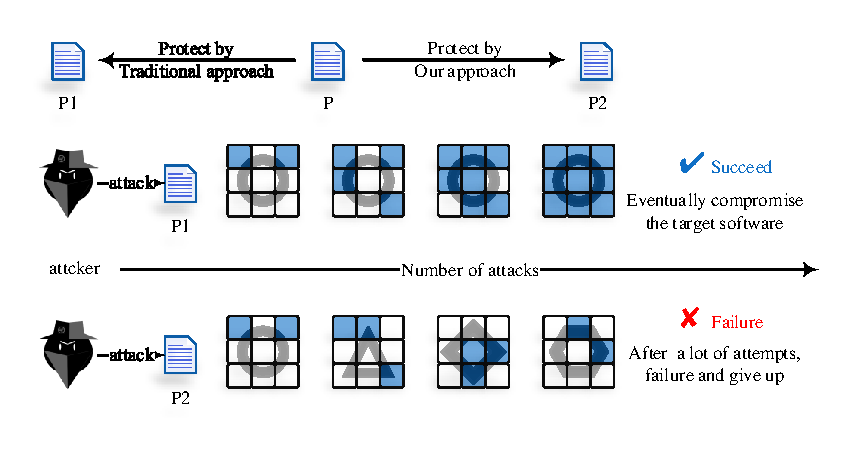
\includegraphics[width=1.0\columnwidth]{figure/figone.pdf}
    \caption{Diversity affects effectiveness of attack. Here a dark small square represents a piece of reusable attacking knowledge. Diverse program execution increases the difficulty of attacks.}\label{fig:Fig.1}
    \vspace{-5mm}
\end{figure}


\section{The Attack Model}
In this work, we assume that the adversary holds an executable binary of the
target software and can run the program in a malicious host
environment~\cite{11collberg2002watermarking}. We also assume the adversary
has the tools and skills to access memory and registers, trace program
instructions, and modify the program instructions and control flows using
tools like ``IDA"~\cite{14Idapro}, ``Ollydbg"~\cite{15Ollydbg} and
``Sysinternals suite"~\cite{16Sysinternalssuite}. The aim of the adversary is
to completely reverse the internal implementation of the target program and
then uses this information to perform attack. Our goal in this work is to
increase the difficulties in terms of time and efforts for an adversary to
reverse the target program implementation using VM-based code obfuscation.



A classical approach to reverse engineer a VM-protected program typically
follows three steps~\cite{10falliere2009inside,17rolles2009unpacking} described as
follows. The first step is
to reverse engineer the two essential components of a VM interpreter: the
dispatcher and bytecode handlers. To do so, the attacker needs to locate
these components and analyze how the dispatcher schedules bytecode
instructions. The second step is to understand how each bytecode is mapped to
machine code. The third step is to use knowledge obtained in the first two
steps to recover the original logical implementation of the target program. A
skilled attacker is able to use knowledge gathered from parts of the program
to analyze other protected regions of the same program or other applications
protected using the same VM scheme and bytecode instructions. In this work,
we assume the attacker has the necessary tools and skills to reuse knowledge
obtained from previous runs of the same program or other programs protected
under the same VM scheme.

\section{Code protection scheme of \DSVMP}
To address the problem of cumulative attacks, we want to introduce a certain
degree of diversity and uncertainty into program execution. This is achieved
through using a diversified scheduling structure (Section~\ref {sec:dvs}) and
multiple VMs (Section~\ref {sec:mvm}) in \DSVMP.
Like other VM-based protection schemes, \DSVMP focuses on
protecting critical code regions to minimize the runtime overhead. %\DSVMP's infrastructure also includes the dispatcher to
%fetch the bytecode instructions.
Figure~\ref{fig:Fig.2} depicts the system architecture of \DSVMP.
Code protection of \DSVMP follows several steps described as follows:

\paragraph*{Code translation}
\DSVMP takes in a compiled program binary and does not require having access to the source code. Code segments need to be protected
are translated into native machine instructions (e.g. x86
instructions) using a disassembler (Step \circled{1}), which will then be mapped into a set of virtual instructions and stored
in the bytecode format (Step \circled{2}).

\paragraph*{Diversifying}
As a departure from prior work on VM-based code obfuscation, \DSVMP employs multiple VM instruction scheduling policies where each scheduler can have more than one dispatcher and each bytecode can be interpreted by more than one handers.
A set of dispatchers and handlers will be randomly chosen from a database to be used for a particular code region (Step \circled{3}). \FIXME{Check this!!}.
Furthermore, each handler will be obfuscated $VMNum$ ($VMNum >= 1$) times by using the deformation engine, resulting in $VMNum$ sets of semantically equivalent bytecode handers with different implementations and control flows (Step \circled{4}).

\textbf{Step5:} Generate \emph{2*VMNum} sets of driver-data. Map VI and handlers then generates \emph{VMNum} sets driver-data (which is composed of the handler's serial number and its parameters.). And the offset value (that between the current handler and next handler) creates the rest of \emph{VMNum} sets driver-data.
\FIXME{I have no idea of what you are talking of here. What are dirver-data, MapVI and why we need to generate 2*VMNum sets of driver-data???!!!}
\textbf{Step6:} Construct the multiple VM, which is composed of the \emph{VMNum} sets of handlers and \emph{2*VMNum} sets of driver-data. \FIXME{Please update steps 5 and 6 and merge this paragraph with the Diversifying paragraph.}

\paragraph*{Code generation}
Finally, a new section will be inserted into the program binary, which contains $VMNum$ VMs and their components such as dispatchers, VMContext etc. It also fills the original code region with junk instructions (Step \circled{7}).
%\par The next few sections elaborate on the above steps, providing the technical details.

This is an overview of our approach. We describe the implementation of \DSVMP in more details in the following sections.

\begin{figure}[t]
  \centering
  % Requires \usepackage{graphicx}
  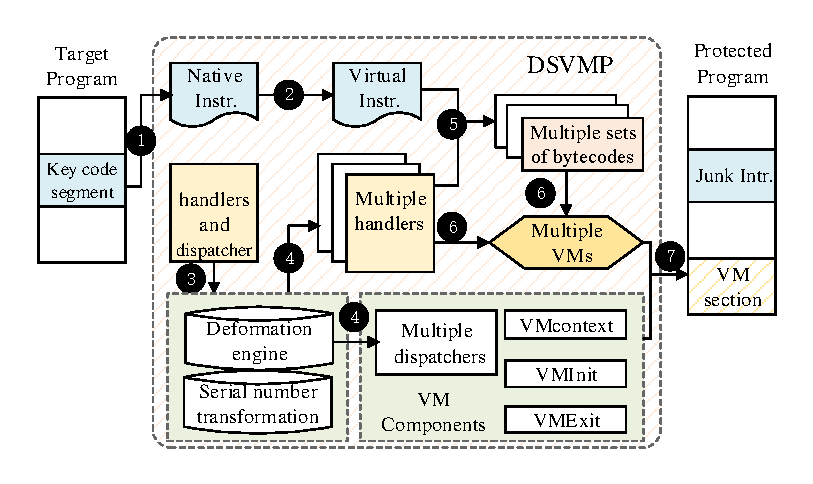
\includegraphics[width=1.0\columnwidth]{figure/figtwo.pdf}
  \caption{Offline code protection process. \DSVMP takes in a program binary. For each protected code region, it translates native instructions into bytecodes. Next, it generates multiple bytecode handlers that are semantically equivalent but implemented in different ways.
  It then generates the corresponding driver-data and multiple VMs. Finally, the generated VMs and associated components will be inserted into the program binary and fills the original code region with junk instructions.}\label{fig:Fig.2}
\end{figure}



\section{\DSVMP Scheduling Structure \label{sec:dvs}}

The \DSVMP VM scheduler uses multiple dispatchers to determine which bytecode instruction should be interpreted at given time.
A unique design of \DSVMP is that the dispatcher used to schedule bytecodes will be dynamically changed at execution time. To further increase
the diversity of program behaviour, \DSVMP also uses multiple  bytecode instruction sets and bytecode handers.

\subsection{Multiple bytecode handlers \label{sec:mb}}

\begin{figure}[t!]
\scriptsize
%\begin{verbatim}
\begin{lstlisting}
lods byte/word/dword ptr ds:[esi]
... ...
push eax
rdtsc                    ;------------------------
mov ecx,2
div ecx                  ;structure control unit
cmp edx,0
jz label                 ;------------------------
lods dword ptr ds:[esi]
... ...                  ; to the next handler
add dword ptr ds:[edi+48],eax
jmp dword ptr ds:[edi+48]
label: push ebx          ;------------------------
div bl
movzx eax,AH             ; return to a dispatcher
add eax,9dH
\end{lstlisting}
\vspace{-2mm}
\caption{Each bytecode handler has a control unit that randomly determines whether the control after exiting the handler should be given to a dispatcher or an alternative bytecode handler. }
\vspace{-5mm}
\label{fig:newhandler}
\end{figure}

In classical VM-based code obfuscation, a single dispatcher is responsible for fetching a bytecode instruction and
determining which bytecode handler should be used to decode the bytecode. Because each bytecode instruction
is decoded by a fixed handler, an adversary can easily work out the mapping of a bytecode instruction and its
handler. From the mapping, the adversary can correlate the native machine code to each bytecode to analyze the
program behavior.

To overcome this issue, for each bytecode handler, we create a number of alternative implementations which all
produce an equivalent output for the same input. The alternative implementations, however,
are implemented in different ways using e.g. different algorithms, data structures or obfuscation methods.
We insert a control unit at the end of each bytecode handler. Before exiting a bytecode handler,
the control unit randomly determines whether the control should be given to a dispatcher or
another handler.

Figure~\ref{fig:newhandler} shows an example of a \DSVMP bytecode handler.
The control unit (lines 4-8) randomly determines to execute the code at line 9 or line 15. \FIXME{Check this!!}
At line 9 , the ``\texttt{lods}" (a load operand in the x86 assembly) instruction fetch an offset value
to calculate the address of an alternative bytecode handler. By contrast, the instruction at line 15 will return
to a dispatcher.


\begin{figure}[t]
  \centering
  % Requires \usepackage{graphicx}
  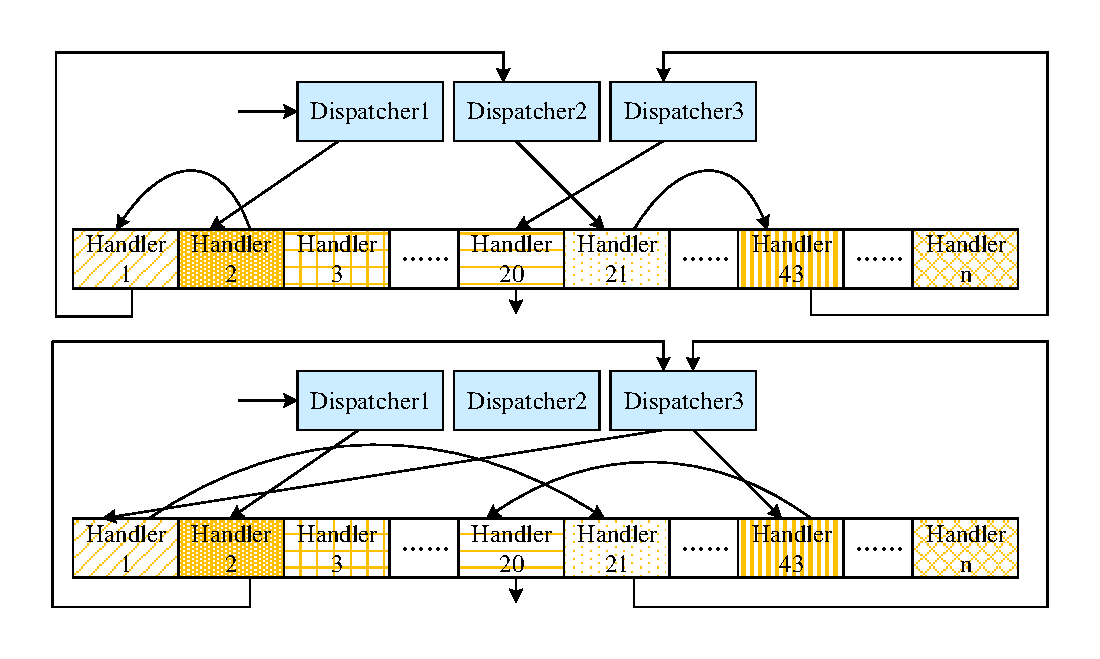
\includegraphics[width=0.45\textwidth]{figure/figdh.pdf}
  \vspace{-1mm}
  \caption{Using multiple dispatchers and handlers increases the diversity of program executions. In this example, the type of handlers and the order of them are called are different across execution runs. }\label{fig:Fig.3}
  \vspace{-5mm}
\end{figure}

\subsection{Multiple bytecode instruction sets and dispatchers \label{sec:mbd}}
As can be seen from Figure~\ref{fig:Fig.2}, the bytecode instruction set
determines the execution order of handlers.
Compared to a single bytecode instruction set, multiple bytecode instruction sets  provide stronger protection because the execution order of
handlers will be more dynamic.
For this reason, \DSVMP uses multiple bytecode instruction sets.

Our current implementation provides two bytecode instruction sets:
\emph{DriverData1} and \emph{DriverData2}. The \emph{DriverData1} is a
standard bytecode instruction sets where each bytecode considers of the
handler's serial number (a ID indicates which bytecode handler should use to
interpret the bytecode) and the operand. \emph{DriverData2} has a different
format compared to  \emph{DriverData1}. The first part of \emph{DriverData2}
is the handler's serial number. The rest of \emph{DriverData2} include the
offset value between two adjacent handlers \FIXME{Which two handlers????} and
the operand.
Recall that a control unit is inserted to the end of each handler. Before exiting the handler, if the control unit chooses to execute the next handler, it will fetch the corresponding offset value from \emph{DriverData2}. They \FIXME{What do they refer to??} are all encrypted.


\DSVMP also provides multiple dispatchers to further increase the diversity
of program execution. As an example, considering Figure~\ref{fig:Fig.3} that
shows two possible program execution using three dispatchers. As can be seen
from the diagram, the type of handlers to be invoked and
the order they are called are different in two different execution runs. Therefore, knowledge about the program control flow extracted from the first run does not apply to the second one.


\section{Multiple VMs \label{sec:mvm}}
\begin{figure}[t!]
  \centering
  % Requires \usepackage{graphicx}
  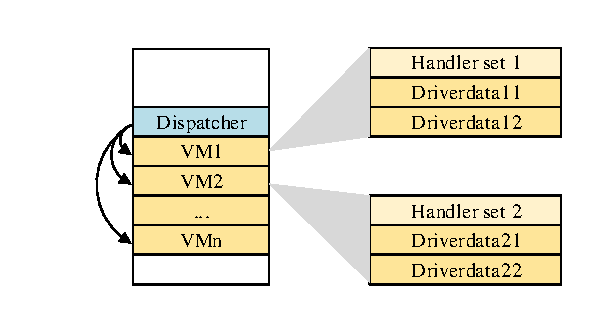
\includegraphics[width=0.8\columnwidth]{figure/figmvm.pdf}\\
  \caption{The structure of multiple VMs. Each VM has one set of unique handlers and two sets of bytecode instructions, \emph{DriverDataSetN1} and \emph{DriverDataSetN2}.}\label{fig:Fig.4}
\end{figure}

In contrast to classical VM-based obfuscation approaches that uses a single
VM (SVM), \DSVMP uses multiple VMs. Multiple VMs offer
different sets handlers and bytecode instruction sets. Under such settings,
bytecode instructions can be scheduled by different VMs and a bytecode instruction can be interpreted by more than one handler.
Therefore, there will be more than one mapping from a bytecode instruction to handlers. Together with the multiple bytecode instruction sets, multiple VMs further increase
the diversity and uncertainly of program execution.


%ZW: I have to comment out this section because it is a such trivial implementation detail!
%\subsection{Generate Multiple Handler sets}
%\emph{HAS} as an original handler set that consists of \emph{n} handlers, it will be obfuscated for \emph{VMNum} times for building multi-VM, then get multiple handler sets and which are semantic equivalence but have different forms. However, all of the equivalent handlers have the same serial number. This is a kind of directly mapping relationship and is detrimental to the security of the system. So further disrupt the serial number of the handler in order to enhance the effect of obfuscation, and the relationship of these equivalent handlers in different sets should be: \emph{HAS$_1$(i)$\Leftrightarrow$HAS$_2$(j)$\Leftrightarrow$ ... $\Leftrightarrow$HAS$_{vm}$(k), }1\emph{$\leqslant$i, j, k$\leqslant$n}, it will produce variety mapping relationship of handler and VI. There are various methods to upset the handler's serial number, we take a simple method that all the serial number plus a uniform random number, then regard the result MOD \emph{m} as the new handler's serial number.
%\par Given the above design, we need to consider one practical issue that is the balance of the security and performance. Depending on the design of the previous section, we need to generate two driver-data sets for each set of handler due to the variety of mapping relationship. So the more the embedded VM number is, the more secure the protected code and the bigger the file size will be.


To schedule the multiple VMs, we need to alter the dispatcher structure. The dispatcher will need to determine which VM to use at runtime.
To do so, we first calculate the address offet between the current VM and the VM to be used. We then store the value of the register \texttt{ESI} and change the pointer of the new bytecode address according to the offset value.
Figure~\ref{fig:Fig.4} shows the multiple VM structure. The VM, the set of bytecode handlers and bytecode instructions will be randomly switched across different code regions in both a single execution and across different program runs.


%All of the dispatchers and handlers will run as the same form after being improved. They all possess the random choice function. It is hard to distinguish two types structure that can enhance the concealment of dispatchers.
%ZW: I comment out because I have no idea what you are talking about!


%ZW: Have no ideas!
%wills random switch driver-data from these VM, if the result is switch to VM2 from VM1, the dispatcher need to adjust value of ESI point to \emph{DriverDataSet21} of VM2 and continue to fetch driver-data to dispatch handler. On the contrary, continue to fetch the driver-data from VM1's \emph{DriverDataSet11} and continue to execute.


\section{Example}

\begin{figure}[t!]
\scriptsize
%\begin{verbatim}
\begin{lstlisting}
STARTSDK
00401036 mov eax, ebx
00401038 sub eax, 03
ENDSDK
\end{lstlisting}
\caption{Example assembly code snippet for a code region to be protected.}
\vspace{-5mm}
\label{fig:examplecode}
\end{figure}


We use the x86 code snippet shown in Figure~\ref{fig:examplecode} as an example to illustrate how \DSVMP operates. \texttt{STARTSDK} and \texttt{ENDSDK} are used to mark the begin and end of the code region respectively, and 00401036 and 00401038 are the address the two assembly instructions.


\subsection{Process of protection}
Firstly, \DSVMP automatically inserts two additional instructions (``\texttt{push 40103B}" abd ``\texttt{ret}") after \texttt{ENDSDK} in order to jump back to execute the native code after the protected code region.
It then converts the native instructions to virtual instructions according to a translation convention. The resulted virtual instructions is given in Table~\ref{tab:Tab.1}.
\DSVMP's bytecode instructions are based on a stack machine model. Here the \texttt{load} instruction is used to push operands into the stack, and the \texttt{store} instruction is used to pop results out from the stack and store the result to the virtual context (VMContext).

\begin{table}[t]
  \centering
  \caption{Generated virtual instructions for the example shown in Figure~\ref{fig:examplecode}.}\label{tab:Tab.1}
  \FIXME{Could you please explain why we have four instructions and what they are?!!!!}
  \scriptsize
\begin{tabular}{|*{3}{p{2cm}|}p{1cm}|}
%{|l|l|l|l|}
  \hline
  % after \\: \hline or \cline{col1-col2} \cline{col3-col4} ...
  \textbf{Ins1} & \textbf{Ins2} & \textbf{Ins3} & \textbf{Ins4}\\
  \hline
  \hline
  \tabincell{l}{\texttt{move 0x08}\\\texttt{load}\\\texttt{move 0x04}\\\texttt{store}} & \tabincell{l}{\texttt{move 0x04}\\ \texttt{load}\\ \texttt{load 0x03}\\ \texttt{sub}\\ \texttt{store}\\ \texttt{move 0x04}\\ \texttt{store}}& \texttt{load 0x40103b} & \texttt{ret} \\
  \hline
\end{tabular}
\vspace{-5mm}
\end{table}

%In this example, we use two VMs: \texttt{VM1} and \texttt{VM2}.
After translating the native code to virtual instructions, we use the deformation engine to transform the bytecode handlers (that will be used to interpret the virtual instructions). For this example, we generate two sets of bytecode handlers which are semantically equivalent but are implemented in different ways.
We also randomly shuffle the serial numbers of these handlers, resulting in two new sets of handlers: \texttt{HAS1} and \texttt{HAS2}.  Each set of bytecode handlers is associated with two bytecode instruction sets: \emph{DriverDataSet11} and \emph{DriverDataSet12} for \texttt{HSA1} and
\emph{DriverDataSet21} and \emph{DriverDataSet22} for \texttt{HSA2}. The resulted program is illustrated in Figure~\ref{fig:Fig.5}. We store the virtual instructions in the bytecode format.
%Transforming the improved handlers using the deformation engine, generating two sets of equivalent but form different handlers, then randomly disturb the serial number and get two new sets of handlers, HAS1 and HAS2. Then, VI was encoded into bytecodes which we call the driver-data.
%According to HAS1, generates the \emph{DriverDataSet11}, which composed of the handler serial number and parameters, illustrated in Figure \ref{fig:Fig.5}. Then built on \emph{DriverDataSet11}, calculate the offset value and get the D\emph{riverDataSet12}. Similarly, According to VM2's HAS2 also can get two sets of driver-data \emph{DriverDataSet21} and \emph{DriverDataSet22}.
%\par Then encrypt four sets of driver-data, the encryption key is kept by register EBX and it will be modified after each encryption.


We also encrypt the resulted bytecode instructions using different keys for different sets of handlers. For example, \emph{DriverDataSet11} and \emph{DriverDataSet12} will be encrypted using one key, and \emph{DriverDataSet21} and \emph{DriverDataSet22} will be encrypted using another key. We fill the code segment to be protected with junk
instructions. Finally, we create a new code section attached to the end of the target program. The new code section contains the implementation of the handlers, different sets of bytecode instructions, dispatchers and other VM components such \texttt{VMContext} and routines such as \texttt{VMInit} (used to initialize the VM) and \texttt{VMExit} (use for cleanup before exiting the VM).



\subsection{Runtime execution}
\begin{figure}[t]
  \centering
  % Requires \usepackage{graphicx}
  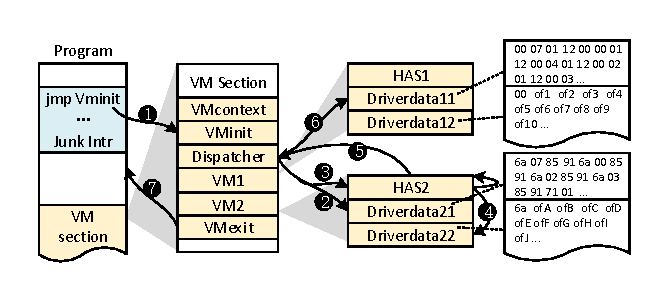
\includegraphics[width=1.0\columnwidth]{figure/figex.pdf}\\
  \caption{The execution process of the protected program. Here each VM has two sets of bytecode instructions and one set of handlers.}\label{fig:Fig.5}
  \vspace{-5mm}
\end{figure}

Runtime execution of the protected code region is illustrated in Figure \ref{fig:Fig.5}, which follows a number of steps:

\begin{itemize}
\item \textbf{Step1:} The entry of the protected code segment contains an ``\texttt{jmp VMInit}" instruction. This transfers the control to the VM initialization routine, \texttt{VMInit}, which saves the host context and initializes the virtual context. The initialized routine also selects a VM scheduler to use. In this example, we assume we use two VMs and \texttt{VM2} is chosen.
\item \textbf{Step2:} Next, a dispatcher starts working. It fetches a bytecode from the \emph{DriverDataSet21}. After decoding, the dispatcher gets an address of ``\texttt{6a}". It then jumps execute ``\texttt{0x6aHandler}" \FIXME{0x6aHandler is not shown in Figure 7??} -- the next bytecode ``\texttt{07}" is its operand.
\item \textbf{Step3:} A control unit will be executed (see Section~\ref{sec:mb}) before exiting the ``\texttt{0x6aHandler}" . The control unit randomly selects to execute another handler, ``\texttt{0x85Handler}", or return the controler to the dispatcher. If it chooses to return to the dispatcher,  the program execution moves to Step 5.
\item \textbf{Step4:} Assume the control unit decides to execute handler, ``\texttt{0x85Handler}". It will then fetch a bytecode from \emph{DriverDataSet21}, decoding it and getting the offset address of ``\texttt{0x85Handler}" . Using the offset, the control unit will jump to \texttt{0x85Handler}. After executing the handler, the program execution moves to Step 3.
\item \textbf{Step5:} If the control unit chooses to return the control to a dispatcher, it will randomly select a dispatcher to continue the execution. This moves to Step 6.
\item \textbf{Step6:} The selected dispatcher randomly selects one VM to use. The dispatcher fetches a bytecode instruction, decoding the instruction to get the handler serial number. The handler serial number tells which handler to use to translate the bytecode to native machine code. It then jumps to execute the handler.  After executing the handler, the program execution moves to Step 3.
\item \textbf{Step7:} Step 3 and Step 4 are iterated until all the bytecodes get executed. The finally step is to invoke the \texttt{VMExit} to restore the native context and to continue executing the target program.
\end{itemize}

\section{Security Strength Analysis}
This section analyzes the security strength provided by \DSVMP. We first analyze the number of possible execution paths. Then we discuss the diversity of code structures.

\subsection{Program execution paths}
Recall that our design goal is to increase the diversity of program execution,
so that in different runts the protected region will not follow a single execution path across runs.
In this analysis, we assume there are 10 different dispatchers. This number matches the current implementation of \DSVMP.
We use the example presented in Section~\ref{sec:mbd} as a case study.
In this example,  \emph{DriverDataSet11} and
\emph{DriverDataSet21} each has 103 bytes of data. They contain a total of 78 handler
serial numbers. In this analysis, we exclude the last handler because of it is used to exit the VM.
This leave us 77 handlers where each handler can lead to 11 different execution paths.
This is because at the end of executing each handler, a control unit will determine whether the control should be given to another handler or one of
the 10 dispatchers (see Section~\ref{sec:mb}) -- 11 possibilities in total.


In combination, these options lead to $11^{77}$ possible execution paths for each protected code region. Therefore,
the probability, $p$, for a protected code region to follow the same execution path across different runs is $p= \frac{1}{{{{11}^{77}}}}$, a very small possibility.
Bear in mind that so far we have  assumed that the protection scheme uses just one VM. The multi-VM strategy employed by \DSVMP further increases
the number of possible execution paths. In fact,  the more dispatchers and VMs are, the greater number of possible execution paths will be.
The current \DSVMP implementation provides five different VMs. Together with the multiple dispatchers and bytecode instruction straggles, for the setting
used in this section, \DSVMP gives a single code region  $11^{385}$ possible execution paths. Given the massive number of choices, it will be rare
for a protected code region to take the same execution path across different runs.



\subsection{Code structures}
To prevent an adversary reuses knowledge obtained from other software to perform attacks, we would like applications protected by \DSVMP exhibit distinct
code structures. In other words, we would like programs after code obfuscation to be as much dissimilar as possible in terms of code structures.

%add new content ֤����ʽ���Ƶ�����
Blietz \emph{et al.}~\cite{18blietz2006software} proposed a method to measure the similarity of program structures, using control flow information such as the number of branches and back blocks, the nesting level of the code etc. We adopt this method to analyze code structures for programs protected using \DSVMP.
We use a number of metrics to describe program code structures. These metrics are:

\begin{itemize}
\item \texttt{NodeNum}: the number of basic blocks of the protected region.
\item \texttt{BranchNum}: the number of basic blocks where the last instruction is a conditional jump instruction.
\item $DR(Vi)$: the number of in and out instructions for the basic block, \emph{Vi}. This metric is defined as $DR(Vi) = {D_{in}}(Vi) + {D_{out}}(Vi)$ where ${D_{out}}\left( {Vi} \right)$ refers to the out-degree and ${D_{in}}\left( {Vi} \right)$ refers to the in-degree.
    \FIXME{What are those in and out degree things?}
\item $DF(Vi)$: the data flow relationship of basic block, \emph{Vi}. This is used to measure the frequency of \emph{Vi}'s information exchange. It is defined as $DF\left( {Vi} \right){\rm{ }} = {\rm{ }}Flo{w_{in}}(Vi) + Flo{w_{out}}(Vi)$, where $Flo{w_{in}}$ is the number of reading instruction in \emph{Vi} and $Flo{w_{out}}$ is the number of writing instruction in \emph{Vi}.
    \FIXME{Why those metrics are not listed in the table???!!! arrrgh!!!! What are the DisNum and VM Num???}
\end{itemize}

\begin{table}
  \centering
    \caption{The relevant information about the program.}\label{tab:Tab.2}
    \scriptsize
  \begin{tabular}{|c|c|c|c|c|c|c|}
%{|p{0.95cm}|p{1.4cm}|p{0.55cm}|p{0.55cm}|p{0.95cm}|p{0.55cm}|p{0.55cm}|}
     \hline
    \multicolumn{4}{|c|}{\textbf{Basic info of target program}}& \multicolumn{3}{|c|}{\textbf{Info of protected-software}} \\
     \hline
     \hline
     % after \\: \hline or \cline{col1-col2} \cline{col3-col4} ...information of protected software
     \textbf{prog.} & \textbf{key code} & \textbf{\tabincell{l}{Dis\\Num}} & \textbf{\tabincell{l}{VM\\Num}} & \textbf{prog.} & \textbf{\tabincell{l}{Node\\Num}} & \textbf{\tabincell{l}{Branch\\Num}}\\
     \hline
     \hline
     A & \tabincell{l}{\texttt{mov eax,ebx}\\ \texttt{sub eax,03}} & 5 & 5 & A' & 23 & 5\\
     \hline
     B & \tabincell{l}{\texttt{pop eax}\\ \texttt{add eax,ebx}} & 10 & 10 & B' & 48 & 9 \\
     \hline
   \end{tabular}
\end{table}

Table~\ref{tab:Tab.2} gives two examples of code regions to be protected and their values of each metric. These are two simple code snippets with just one basic block and no branches. Without code obfuscation, these two examples have very similar structures because \FIXME{XX?? WHY??}. Transforming the code regions using \DSVMP, we obtain different metric values for both code regions, which indicate the transformed code segments
have distinct structures. We use the following formula to quantify the code structure information, X after code obfuscation.

\[\begin{array}{l}
 SInfo{r_{X}} = NodeNu{m_{X}} + BranchNu{m_{X}} \\
                                                 + \sum\limits_{i = 0}^{i < n} {(DR(i) + DF(i))}
 \end{array}\]

Applying this formula for the transformed code segments, A' and  B', listed in Table~\ref{tab:Tab.2},  we get :

\[\begin{array}{l}
 SInfo{r_{A'}} = NodeNu{m_{A'}} + BranchNu{m_{A'}} \\
                                                 + \sum\limits_{i = 0}^{i < n} {(DR(i) + DF(i))} \\
                                       = 23 + 5 + (DR(0) + DR(1) + ... + DR(22) \\
                                                 + DF(0) + DF(1) + ... + DF(22)) \\
                                       = 92 \\
 SInfo{r_{B'}} = NodeNu{m_{B'}} + BranchNu{m_{B'}} \\
                                                 + \sum\limits_{i = 0}^{i < m} {(DR(i) + DF(i))}  \\
                                        = 48 + 9 + (DR(0) + DR(1) + ... + DR(47) \\
                                                + DF(0) + DF(1) + ... + DF(47)) \\
                                        =  189
\end{array}\]


From $SInfo{r_{A'}}$ and $SInfo{r_{B'}}$, we can calculate the similarity of code structure, $SDiff$, for A' and B' as:
\[SDiff = \frac{{|SInfo{r_{A'}} - SInfo{r_{B'}}|}}{{SInfo{r_{A'}} + SInfo{r_{B'}}}}\;{\kern 1pt}  = \frac{{97}}{{281}} = 34.5\% \]

Thus it can be seen the code structure similarity between two A' and B' is  34.5\%. This example shows that \DSVMP can significantly
increase the dissimilarity of code structures even for simple code segments.  We also observe that the similarity between transformed code
regions drops significantly as the complexity of original code segments increases.

\section{Performance Evaluation}
%In this section, we first discusse the experimental and cost analysis, and then present the evaluation results of \DSVMP based on the experimental data in detail.

\subsection{Experimental Setup}
In our experiments, we used three VMs and five dispatchers for \DSVMP.
\DSVMP building upon IDA~\cite{14Idapro} an existing code obfuscation tool. \DSVMP uses IDA to process the program binary to locate the  code segment to protect and to obtain the control flow graph of the protected code region.
%after into the virtual machine, but the last one basic block ended in an indirect jump instruction, "IDA" can not automatic acquisition the target address, so it is incomplete.
%We also collected the dynamic instructions, and then manually connect the basic block to draw a complete control flow graph.
%By utilizing taint analysis and control dependencies to simplify and extract the software structure information. But the control flow structure has changed when we try to analyze the software again, previous attack experience is useless, we can only take time again to draw complete control flow graph in current state.

\DSVMP also uses OllyDbg~\cite{15Ollydbg} to perform the dynamic debugging, and then locate the dispatcher. It uses the x86 register \texttt{ESI} as the program counter (PC) for bytecode instruction. \DSVMP also uses \texttt{ESI} to track the movement of tainted data.
\DSVMP uses another register \texttt{EAX} to store the memory address of a decrypted bytecode instruction together with the serial number of the handler used
to decode the instruction. Collect all values that scheduled by each dispatcher, as follows:
%\begin{verbatim}
%00 0A 12 15 37 64 00 0A 12 89 0B 02 57 36
%78 9A 8E 65 0C 13 25 32 11 24 0A 12 24 8F
%4E 35 34 01 02 07 12 24 09 2A 31 44 05 01
%0F 12 34 52 35 09 01 65 81 33 01 0A 07 12
%34 25 36 93 78 32 57 04 05 01 30 4C 3D 67
%13 45 21 01 03 07
%\end{verbatim}

%%%%
%% I really don't know what those numbers are!!! I comment them out because I don't know how to explain them!!!!
%\begin{verbatim}
%00 0A 12 15 37 64 00 0A 12 89 0B 02 57 36
%78 9A 8E 65 0C 13 25 32 11 24 0A 12 24 8F
%4E 35 34 01 02 07 12 24 09 2A 31 44 05 01
%0F 12 34 52 35 09 ... ...
%\end{verbatim}
%\par But these serial numbers are composed of multiple VM, and it is incomplete because some handlers did not schedule through the dispatcher. So it is difficult to distinguish the relationship between these handler serial numbers and VMID. \DSVMP embed multiple sets of handler in virtual interpreter, the attacker wants to analyze these handler completely is very difficult. Even it can be fully analyzed, we still unable to crack the software, because we don't know the relationship of handler serial number and set of handler.

\subsection{Evaluation platform and benchmarks}
We evaluated \DSVMP on a PC with an 3.0 GHz Intel Core$^{TM}$ 2 Duo processor with 4GB of RAM.
The PC runs Windows 7 operating system. We evaluated our approach using four widely use applications: \texttt{md5}~\cite{19md5}, \texttt{aescrypt}~\cite{20Aescrypt}, \texttt{bcrypt}~\cite{21bcrypt} and \texttt{gzip}~\cite{22gzip}.
 We used these applications to process a test image file. The size of the file is 763 KB.
 Table~\ref{tab:Tab.3} gives information of the protected code regions for each benchmark.
 The 3rd column of the table gives the function to be projected and the 4th column shows the number of instructions of the function at the program binary.
 Finally, the number of instructions got executed with the functions while processing the test file is shown in the last column of the table.

\begin{table}
  \centering
    \caption{Information of the bechmarks.}\label{tab:Tab.3}

  \begin{tabular}{|l|r|l|r|r|}
     \hline
     % after \\: \hline or \cline{col1-col2} \cline{col3-col4} ...information of protected software
     \textbf{prog.} & \textbf{Size(KB)} & \textbf{Func. to protect} & \textbf{\tabincell{l}{Instr.\\Protect}} & \textbf{\tabincell{l}{Instr.\\Executed}}\\
     \hline
     md5 & 11 & \texttt{Transform} & 563 & 6869163\\
     \hline
     aescrypt & 142 & \texttt{encrypt-stream} & 1045 & 5502747\\
     \hline
     bcrypt & 68 & \texttt{Blowfish-Encryp}t & 54 & 43945017\\
     \hline
     gzip & 56 & \texttt{deflate} & 154 & 35877278\\
     \hline
   \end{tabular}
\end{table}

\begin{figure}[t]
\centering
\subfloat[][]{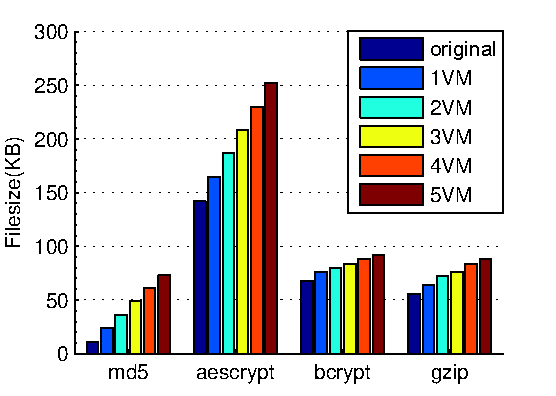
\includegraphics[width=.24\textwidth]{figure/fig6a.pdf}}
\subfloat[][]{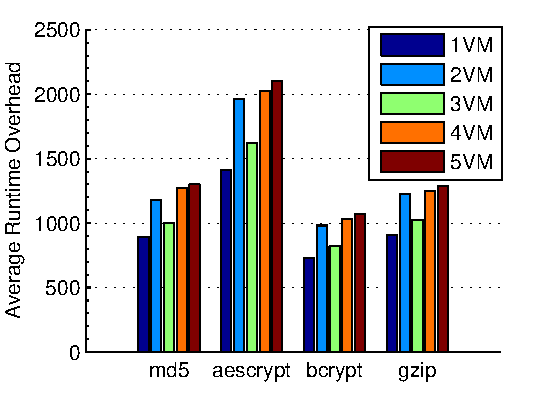
\includegraphics[width=.24\textwidth]{figure/fig6b.pdf}}
\caption{(a) The impact of code sizes (KB) for configurations with a different number of VMs. (b) The average runtime overhead per instruction with different VMs.}\label{fig:Fig.6}
\centering
\subfloat[][]{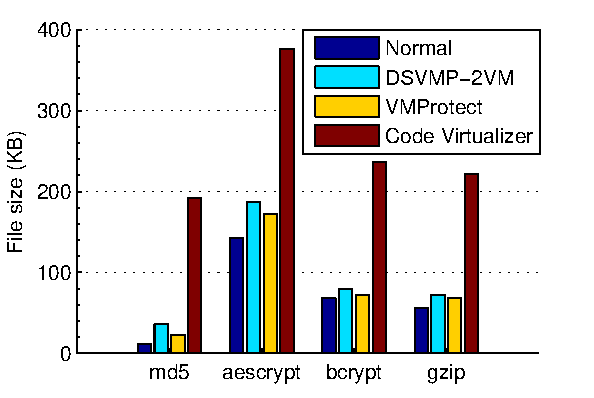
\includegraphics[width=.24\textwidth]{figure/fig7a.pdf}}
\subfloat[][]{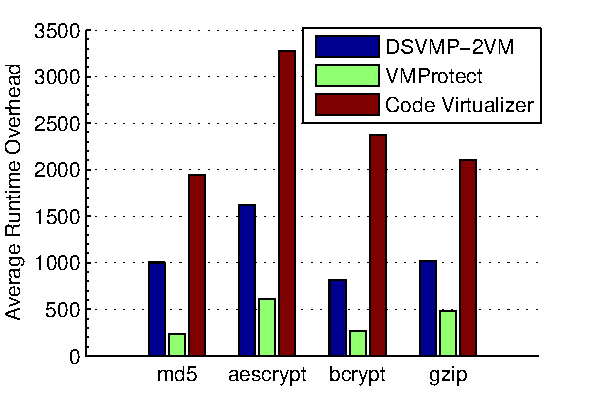
\includegraphics[width=.24\textwidth]{figure/fig7b.pdf}}
\caption{(a) The comparison of impact on file size (KB) with VMProtect and Code Virtualizer. (b) The comparison of average runtime overhead per dynamically executed critical instruction with VMProtect and Code Virtualizer.}\label{fig:Fig.7}
\vspace{-2mm}
\end{figure}


\subsection{Code Size and Runtime Overhead}
\paragraph*{Code size} For each target benchmark, we applied \DSVMP to the target function and repeated the process for five times. For each protection run, we used a different number of VMs. Figure~\ref{fig:Fig.6} (a) shows how the \DSVMP multi-VM scheme affects the code size.
 As described before, each VM has two bytecode instruction sets and one set of handlers, the code size of the protected program grows as the number of VM increases. Moreover, there is a strong correlation between the code size of and the number of instructions after code obfuscation.  This explains why \texttt{aescrypt} has the fastest increase of code size as it has the largest number of instructions after code obfuscation (see Table~\ref{tab:Tab.3}.
  For the same reason, the code size of \texttt{bcrypt} grows slower than other programs, as this benchmark has the least number of instructions after code obfuscation.

\paragraph*{Runtime overhead} To evaluate the runtime overhead of \DSVMP, we used each benchmark to process the file. We repeated the process for 10 times and report the average runtime overhead per instruction. The results are shown in Figure~\ref{fig:Fig.6} (b).
As can be seen from this diagram, the runtime overhead increases as the number of VM used increases. The only exception is that the 3-VM configuration (3VM) has a lower overhead than a 2-VM one. One possible reason is that the implementation strategy we used for multi-VM protection. \FIXME{This doesn't explain anything. Why the implementation strategy leads to this?}
Furthermore, \texttt{aescrypt} has a much higher runtime overhead than other benchmarks. The \texttt{encrypt-stream} function of  \texttt{aescrypt} is  more complex and thus has a higher number of virtual instructions compared to other benchmarks. As such, it takes longer to execute the obfuscated code for this program compared to other benchmarks.

\subsection{Comparisons with state-of-the-arts}
We also compared \DSVMP against two commercial VM protection systems, Code Virtualizer (CV)~\cite{2CV} and VMProtect~\cite{3Vmprotect}, in terms of code sizes and runtime overhead.
We use the FISH32 (White) VM from the 24 customized VMs of CV to perform code protection because this VM has least runtime overhead. We used a configuration of two VMs for \DSVMP, \DSVMP-2VM, in this experiment.

\paragraph*{Code size} Figure \ref{fig:Fig.7} (a) shows the impact on code size of three different VM-based protection systems. The code size of programs protected under CV grows faster than the other two schemes. However, the resulted code size of CV is relatively stable across benchmarks. On the other hand, the code sizes of \DSVMP and VMProtect are comparable and smaller than CV.


\paragraph*{Runtime overhead}
Figure \ref{fig:Fig.7} (b) shows the average runtime overhead of the three schemes. Code protected under CV has the most expensive runtime overhead, which on average is 2x higher than \DSVMP. Among the three schemes, VMProtect has the smallest overhead while \DSVMP has a slightly higher overhead compared to VMProtect.
Consider that \DSVMP provides stronger protection with a diverse set of handlers, dispatchers and VMs, we argue that the modest increase in runtime overhead is acceptable.


\section{Related Work}
Early work on the binary code protection relies on simple encryption and obfuscation methods, but they are vulnerable to the sophisticated, diversified attacks developed over the past years.
Traditionally, techniques like junk instructions~\cite{23linn2003obfuscation}, packers~\cite{25Execryptor,26upx}, are used to protect software against attacks based on disassembly and static analysis.
There are also other code protection techniques like code obfuscation~\cite{25wu2010mimimorphism}, control flow and data flow obfuscation~\cite{13liem2008compiler,27ge2005control,27balachandran2014function},  all aim to obfuscate the semantic and logical information of the target program.
In practice, these approaches are often used in combination  to provide stronger protection. \DSVMP also leverages some of the code obfuscation techniques developed in the past for code protection.


There is a growing interest in using code virtualization to protect software from malicious reverse engineering.
Fang \emph{et al.}~\cite{5fang2011multi} proposed a protection scheme based on multi-stage code obfuscation. Their approach iteratively transforms the critical code region  several times  with different interpretation methods to improve security.
Yang \emph{et al.}~\cite{6ming2011software} presented a nested virtual machine for code protection. Using their approach, an adversary would have to fully reverse engineer a layer of the interpreter before moving to the next layer, which increases the cost of attacks.
Averbuch \emph{et al.}~\cite{27averbuch2011efficient} introduces an encryption and decryption technology on the basis of VM-based protection. This approach uses the AES algorithm and a customize encryption key to encrypt the virtual instructions. During runtime, the VM  will decrypt the virtual instruction and then dispatch a handler to interpret the virtual instructions.
Wang \emph{et al.}~\cite{7wang2014tdvmp} proposed a protection scheme to increase the time diversity of protected code regions. This is achieved by constructing several equivalent but different forms of sub program execution paths, from which a path will be randomly selected to execute at runtime.

As a departure from prior work, \DSVMP presents a dynamic scheduling structure to improve security for software.
\DSVMP has integrated several novel techniques to increase the diversity and uncertainly of program execution. These include using a control unit to diversify the execution path of bytecode handlers and using multiple VMs and dispatchers to randomly schedule instructions from multiple bytecode instruction sets.
Integrating these techniques allows \DSVMP to provide a more diverse program execution structure compared to prior work in the area. This richer set of diversity can better protect software against code reverse engineering~\cite{20larsen2014sok}.


\section{Conclusions}
This paper has presented \DSVMP, a novel VM-based code protection scheme.
\DSVMP uses a dynamic scheduling structure and multiple VMs to increase
diversity of program execution. We have shown that code
segments protected by \DSVMP rarely follow the same execution path across
different runs. The dynamic program execution brought by \DSVMP forces the attacker
to have to use many trail runs to uncover the implementation of the protected code
region. As such, \DSVMP significantly increases the overhead and effort
involved in code reverse engineering. We have evaluated \DSVMP using four
real world applications and compared it to two state-of-the-art VM-based code
protection schemes. Our experimental results show that \DSVMP provide
stronger protection with comparable overhead of runtime and code
size.
%
%In this paper, we introduce the details of improved VM-based protection called \DSVMP, it proposes improved diversity scheduling structure and multiple VM to mitigate the vulnerability of the classical VM. We show the implementation process of our system, and we also analyze and evaluate that our \DSVMP is practical and effective for resilient the dynamic accumulation attacks.
%\par \DSVMP also has vulnerability, multi-VM randomly selected by the dispatcher's selection structure, and in MVM, each VM can independently finish the complete function. Although the handler also has a random select structure that improves the concealment of dispatcher, once the adversary locates the dispatcher, they can tamper with the control structure to affect the results of selection, so that MVM will be failure.
%\par We intend to increase the tamper-proof technology into our system. Further, we can add a security thread library, contains of the anti-debug and anti-dump threads etc. We also can improve the virtual instruction set and driver-data to make each VM only contains part of the whole driver-data, so that the adversary has to analyze the different VMs.
% conference papers do not normally have an appendix

% use section* for acknowledgment
\section*{Acknowledgment}
This work was partial supported by projects of the National Natural Science Foundation of China (No. 61373177, No. 61572402), the Key Project of Chinese Ministry of Education (No. 211181), the International Cooperation Foundation of Shaanxi Province, China (No. 2013KW01-02, No. 2015KW-003, No. 2016KW-034), the China Postdoctoral Science Foundation (grant No. 2012M521797), the Research Project of Shaanxi Province Department of Education (No. 15JK1734), the Research Project of NWU, China (No. 14NW28), and the UK Engineering and Physical Sciences Research Council under grants EP/M01567X/1 (SANDeRs), EP/M015793/1 (DIVIDEND).

%The authors would like to thank...

% trigger a \newpage just before the given reference
% number - used to balance the columns on the last page
% adjust value as needed - may need to be readjusted if
% the document is modified later
%\IEEEtriggeratref{8}
% The "triggered" command can be changed if desired:
%\IEEEtriggercmd{\enlargethispage{-5in}}

% references section

% can use a bibliography generated by BibTeX as a .bbl file
% BibTeX documentation can be easily obtained at:
% http://mirror.ctan.org/biblio/bibtex/contrib/doc/
% The IEEEtran BibTeX style support page is at:
% http://www.michaelshell.org/tex/ieeetran/bibtex/
%\bibliographystyle{IEEEtran}
% argument is your BibTeX string definitions and bibliography database(s)
%\bibliography{IEEEabrv,../bib/paper}
%
% <OR> manually copy in the resultant .bbl file
% set second argument of \begin to the number of references
% (used to reserve space for the reference number labels box)

%\begin{thebibliography}
%\bibitem{IEEEhowto:kopka}
%H.~Kopka and P.~W. Daly, \emph{A Guide to \LaTeX}, 3rd~ed.\hskip 1em plus
%  0.5em minus 0.4em\relax Harlow, England: Addison-Wesley, 1999.

\bibliographystyle{IEEEtran}
\bibliography{reference}

%\end{thebibliography}14Ida pro14Ida pro14Ida pro14Ida pro
% that's all folks
\end{document}


